\section{Task 2: Tree-Code}

\begin{frame}{Multipole Expansion}
	\begin{columns}
		\column{.5\linewidth}
		\begin{itemize}
			\item $\vb{r}$ is sufficiently far
			      away
			\item  Seen under small opening angle
			      $\theta$
			\item  Orders of multipole corrections
		\end{itemize}
		\column{.5\linewidth}
		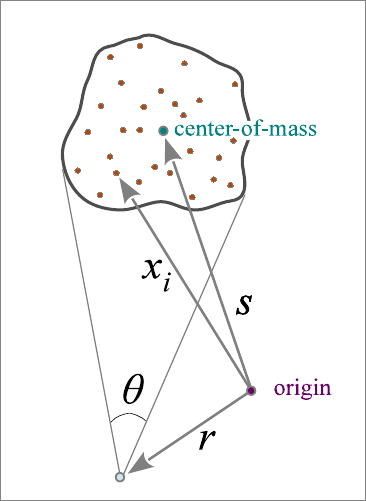
\includegraphics[width=\linewidth]{figures/multipole.png}
	\end{columns}
\end{frame}

\begin{frame}{Multipole Moments}
	\begin{itemize}
		\item Monopol
		      \begin{equation}
			      M = \sum_i m_i
		      \end{equation}
		\item Center of Mass
		      \begin{equation}
			      \vb{s} = \frac{1}{M}\sum_im_i\vb{x_i}
		      \end{equation}
		\item Quadrupol ($\vb{Q} \in \mathbb{R}^{3\times3}$)
		      \begin{equation}
			      \vb{Q}_{i j}=\sum_k m_k\left[3\left(\mathbf{s}-\mathbf{x}_k\right)_i\left(\mathbf{s}-\mathbf{x}_k\right)_j-\delta_{i j}\left(\mathbf{s}-\mathbf{x}_k\right)^2\right]
		      \end{equation}
	\end{itemize}
\end{frame}

\begin{frame}{Gravitational Potential \& Force}
	\begin{itemize}
		\item Potential:
		      \begin{equation}
			      \Phi(\mathbf{r_i})=-G\left(\frac{M}{|\mathbf{y}|}+\frac{1}{2} \frac{\mathbf{y}^T \mathbf{Q} \mathbf{y}}{|\mathbf{y}|^5}\right), \quad \mathbf{y}=\mathbf{r}_i-\mathbf{s}
		      \end{equation}
		\item Monopole Force:
		      \begin{equation}
			      \vb{F}_M(\vb{r}_i) = - \frac{m_i  M}{ | \vb{y} | ^3}\vb{y}
		      \end{equation}
		\item Quadrupole Force:
		      \begin{equation}
			      \vb{F}_Q(\vb{r}_i) = \frac{\vb{Q}\vb{y}}{ | \vb{y} | ^4} - \frac{5}{2} \frac{\vb{y}^T \vb{Q} \vb{y}} { | \vb{y} | ^4} \vb{y}
		      \end{equation}
		\item Total Force:
		      \begin{equation}
			      \vb{F}(\vb{r}_i) = \vb{F}_M + \vb{F}_Q
		      \end{equation}
	\end{itemize}
\end{frame}


\begin{frame}{Hierarchical Grouping}
	\begin{columns}
		\column{.35\linewidth}
		\begin{itemize}
			\item Octree
			\item Axis-aligned cubes
			\item Every particle is a leaf node
			\item Empty cubes not stored
			\item Children have $c^\prime = \frac{1}{2}c$ side length
		\end{itemize}
		\column{.65\linewidth}
		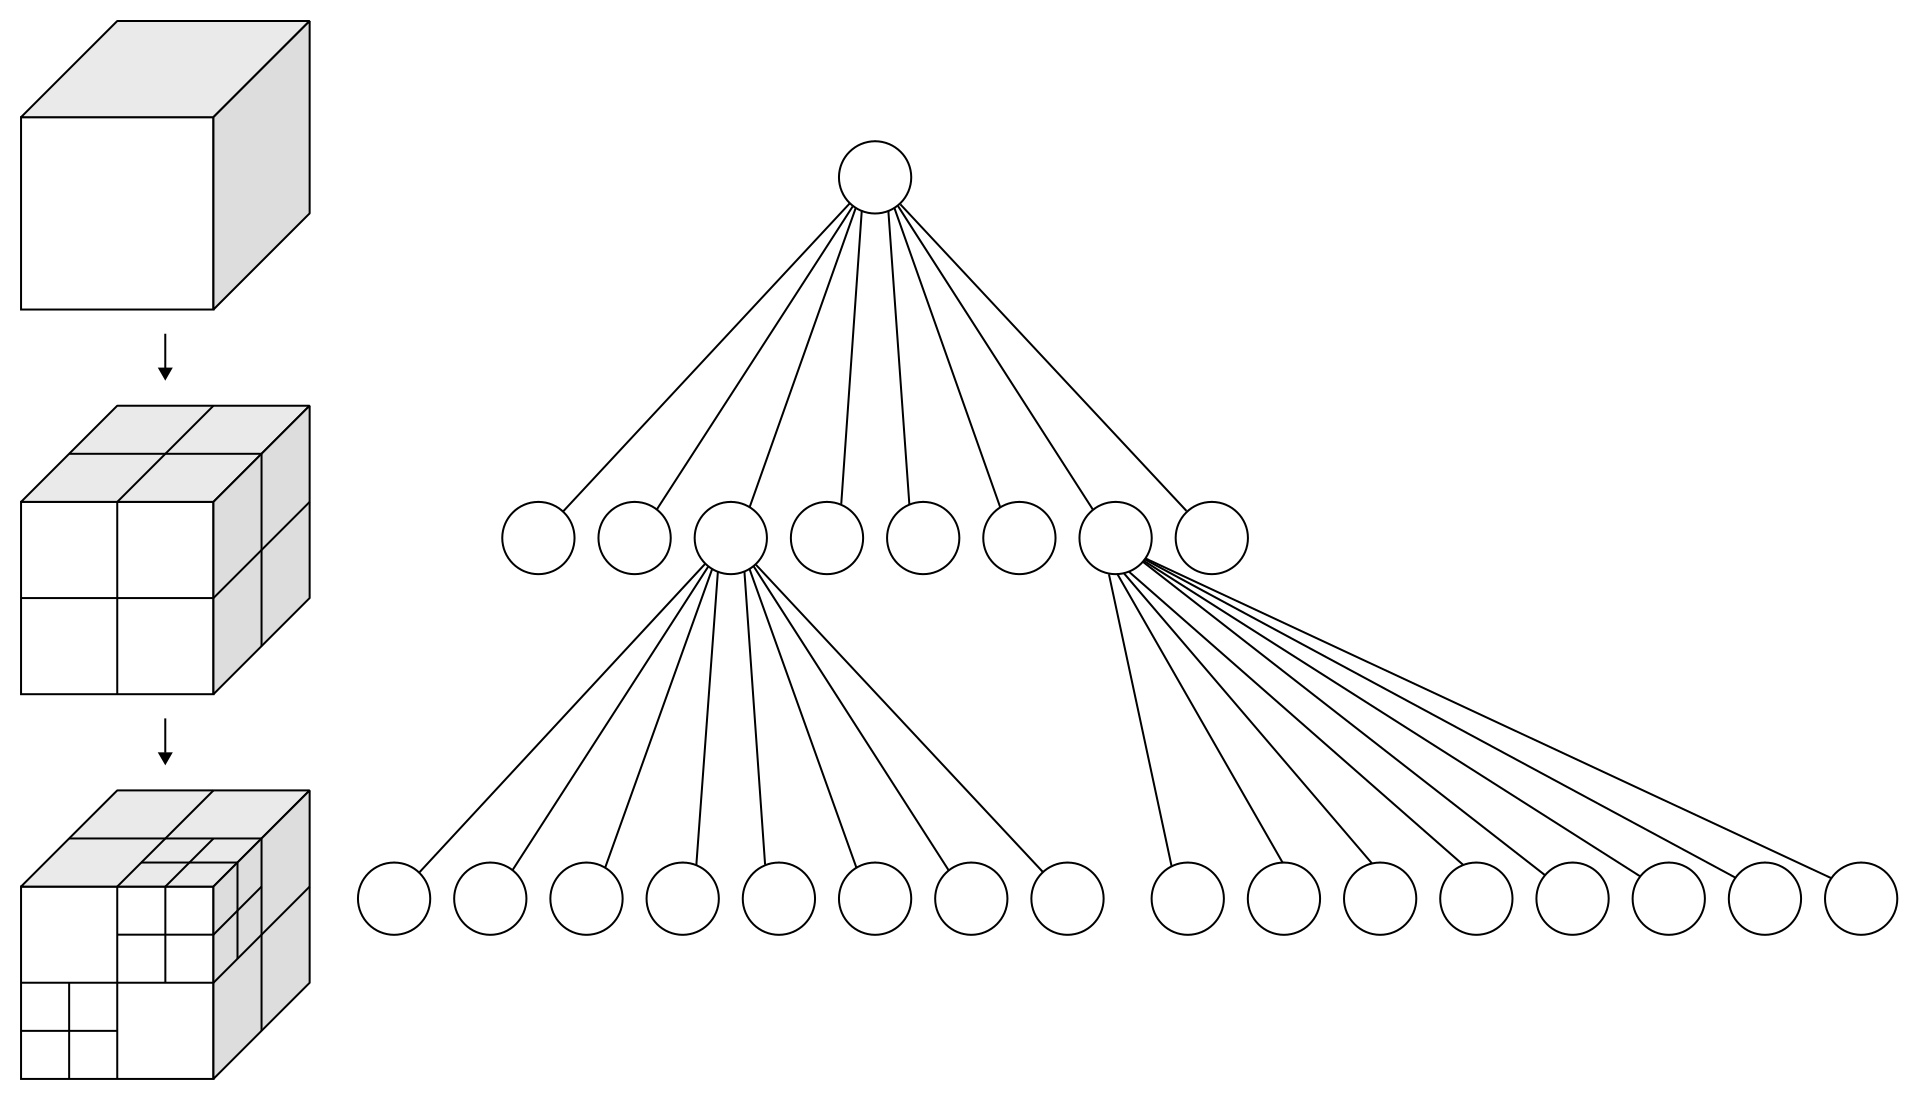
\includegraphics[width=\linewidth]{figures/cube.png}
	\end{columns}
\end{frame}

\begin{frame}[plain]{Octree}
	\includegraphics[width=\textwidth]{figures/plots/treecode.png}
\end{frame}

\begin{frame}{When to apply the expansion?}
	\begin{itemize}
		% arctangent (inverse tangent) of the ratio of two specified numbers,
		% TODO: (aver) just just `arctan` instead of atan2 for the presentation
		\item Opening angle:
		      \begin{equation}
			      \theta \simeq \operatorname{std::atan2}\left({c, |\vb{y}| }\right)
		      \end{equation}
		\item Tolerance Angle $\theta_c$
		\item In the limit $\theta_c \rightarrow 0$  direct summation force.
	\end{itemize}
\end{frame}

\begin{frame}{Tree Walk}
	\begin{itemize}
		\item Depth-First traversal
	\end{itemize}
	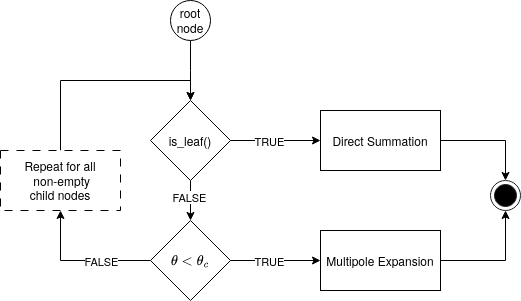
\includegraphics[width=0.95\textwidth]{figures/multipole_uml.png}
\end{frame}

\begin{frame}{Force Comparison}

\end{frame}

